% Enable warnings about problematic code
\RequirePackage[l2tabu, orthodox]{nag}

\documentclass{WeSTassignment}

% The lecture title, e.g. "Web Information Retrieval".
\lecture{Introduction to Web Science}
% The names of the lecturer and the instructor(s)
\author{%
  Prof. Dr.~Steffen~Staab\\{\normalsize\mailto{staab@uni-koblenz.de}} \and
  Ren{\'e}~Pickhardt\\{\normalsize\mailto{rpickhardt@uni-koblenz.de}} \and
   Korok~Sengupta\\{\normalsize\mailto{koroksengupta@uni-koblenz.de}}
}
% Assignment number.
\assignmentnumber{6}
% Institute of lecture.
\institute{%
  Institute of Web Science and Technologies\\%
  Department of Computer Science\\%
  University of Koblenz-Landau%
}
% Date until students should submit their solutions.
\datesubmission{December 6, 2016, 10:00 a.m.}
% Date on which the assignments will be discussed in the tutorial.
\datetutorial{December 9, 2016, 12:00 p.m.}

% Set langauge of text.
\setdefaultlanguage[
  variant = american, % Use American instead of Britsh English.
]{english}

% Specify bib file location.
\addbibresource{bibliography.bib}

% For left aligned centerd boxes
% see http://tex.stackexchange.com/a/25591/75225
\usepackage{varwidth}

% ==============================================================================
% Document

\begin{document}

\maketitle
Please look at the lessons 1) \textbf{Simple descriptive text models} \& 2) \textbf{Advanced descriptive text models}

For all the assignment questions that require you to write code, make sure to include the code in the answer sheet, along with a separate python file. Where screen shots are required, please add them in the answers directly and not as separate files.\\ \\ 

%Please mention your team Names here: 
Team Name: Echo

% ------------------------------------------------------------------------------
\section{Digging deeper into Norms (10 points)}

You have been introduced to the concept of a norm and have seen that the uniform norm $|| \cdot ||_\infty$ fullfills all three axioms of a norm which are:

\begin{enumerate}
\item Positiv definite
\item Homogeneous
\item Triangle inequality
\end{enumerate}

Recall that for a function $f:M\longrightarrow \mathbb{R}$ with $M$ being a finite set\footnote{You could for example think of the function measuring the frequency of a word depening on its rank.} we have defined the $L_1$-norm of $f$ as:

\begin{equation}
|| f ||_1 := \sum_{x\in M}|f(x)|
\end{equation}

In this exercise you should
\begin{enumerate}
\item calculate $||f - g||_1$ and $||f -g||_\infty$ for the functions $f$ and $g$ that are defined as \begin{itemize}
\item $f(0) = 2, f(1) = -4, f(2) = 8, f(3) = -4$ and 
\item $g(0) = 5, f(1) = 1, g(2) = 7, g(3) = -3$ \end{itemize}
\item proof that all three axioms for norms hold for the $L_1$-norm.
\end{enumerate}


\subsection{Hints:}
\begin{enumerate}
\item The proofs work in a very similar fashion to those from the uniform norm that was depicted in the videos. 

\item You can expect that the proofs for each property also will be "three-liners".

\item Both parts of this exercise are meant to practice proper and clean mathematical notation as this is very helpfull when reading and understanding research papers. Discuss in your study group not only the logics of the calculation and the proof (before submission) but try to emphasize on the question whether your submission is able to communicate exactly what you are doing. 

\end{enumerate}

\textbf{Answer:} \\
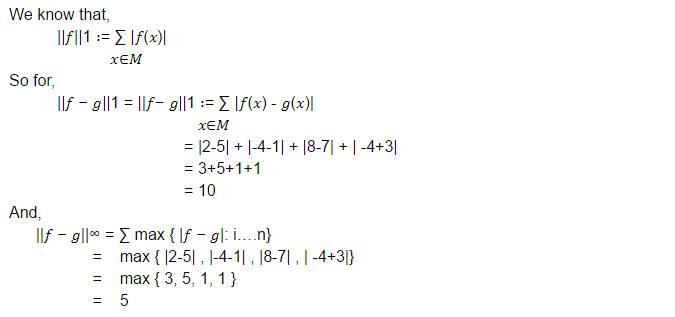
\includegraphics[width=1\textwidth]{1_new1.png}
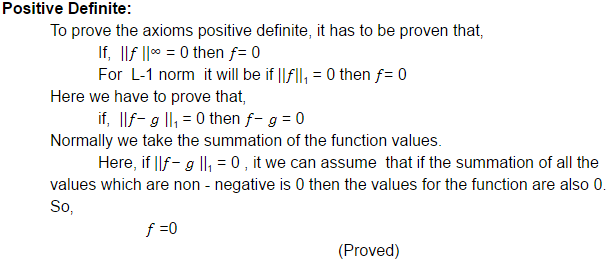
\includegraphics[width=1\textwidth]{2.png}
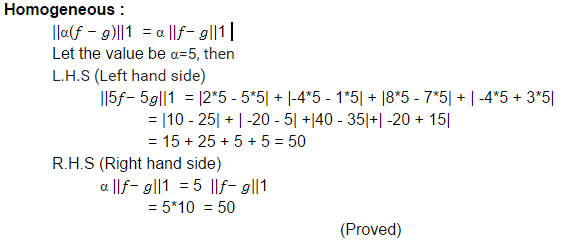
\includegraphics[width=1\textwidth]{3.png}
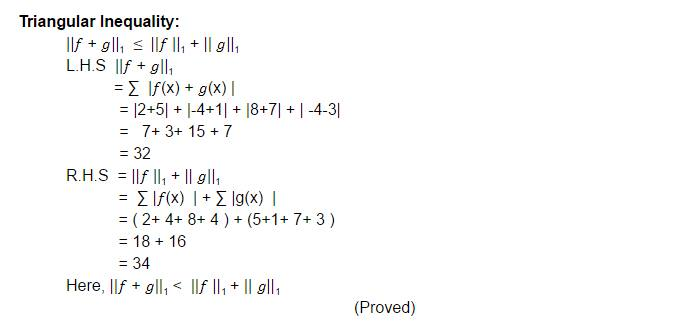
\includegraphics[width=1\textwidth]{4_new.png}

% ------------------------------------------------------------------------------
\section{Coming up with a research hypothesis (12 points)}
You can find all the text of the articles from Simple English Wikipedia at \url{http://141.26.208.82/simple-20160801-1-article-per-line.zip} each line contains one single article. 

In this task we want you to be creative and do some research on this data set. The ultimate goal for this exercise is to practice the way of coming up with a research hypothesis and testable predictions. 

In order to do this please \textbf{shortly}\footnote{Depending on the question shortly could mean one or two sentences or up to a thousand characters. We don't want to give a harsh limit because we trust in you to be reasonable.} answer the following questions: 

\begin{enumerate}
\item What are some obervations about the data set that you can make? State at least three obervations.
\item Which of these observations make you curious and awaken your interest? Ask a question about why this pattern could occur.
\item Formulate up to three potentiel research hypothesis.
\item Take the most promesing hypothesis and develop testable predictions.
\item Explain how you would like to use the data set to test the prediction by means of descriptive statistics. Also explain how you would expect your outcome. 

(If you realize that the last two steps would not lead anywhere repeat with one of your other research hypothesis.)
\end{enumerate}

\subsection{Hints:}
\begin{itemize}
\item The first question could already include some diagrams (from the lecture or ones that you did yourselves).
\item In step 3 explain how each of your hypothesis is falsifiable. 
\item In the fifth step you could state something like: "We expect to see two diagrams. The first one has ... on the x-axis and ... on the y-axis. The image should look like a ... The second diagram ...". You could even draw a sketch of the diagram and explain how this would support or reject your testable hypothesis. 
\end{itemize}

\textbf{Answer:} \\
1.Observations: \\
After observing the first 10-20 articles in the dataset: \\
\begin{itemize}
\item In this dataset, computer science terms occurances are so less. \\
\item In this dataset, each article has a specific topic \\
\item This dataset contains more articles with positive affect than negative \\
\item This dataset does not contain any non-english words \\ \\
\end{itemize}
2.Explain One observation: \\
In this dataset, computer science terms occur so less.\\
To find the average percentage of computer science terms occurance in all articles in the dataset is interesting because then we know how frequent it is to have computer science terms distributed in different kinds of article topics. \\ \\

3. Three Hypothesises FOR "In this dataset, computer science terms occurances are so less" \\
\begin{itemize}
\item Computer science words occurances are less than 30\% in all articles in the dataset \\
Falsible: Computer science words occurances are more than 30\% in all articles of the dataset \\
\item Computer science words occurances are less than 30\% in each article in terms of all words in each article \\
Falsible: Computer science words occurances are more than 30\% in each article in terms of all words in each article \\
\item Computer science related articles are less than 20\% in the dataset than other topics. \\
Falsible: Computer science related articles are more than 20\% in the dataset \\ \\
\end{itemize}
4.Testable prediction FOR "1. Computer science words occurances are less than 30\% in all articles in the dataset" \\
(a) The average percentage of the computer science terms (the list given in computer.txt) in the dataset will be less than (30\%) The percentage that we are predicting of computer science terms in the dataset is less than 30\%. In our case we have chosen to check the distribution of computer science terms in the dataset, and that is justified by counting the number of computer science terms occurances in each article over the number of all words in the article. Then sum all the percentages. \\ \\
5.Plan: \\
\begin{itemize}
\item We will go through each article, find the average amount of computer science terms (from the list in computer.txt) in each article. \\
\item Collect in a dictionary the average amount of computer science words in each article, then sum up all percentages to find the average percentage of the occurances of computer science terms in all the dataset \\
\end{itemize}
% ------------------------------------------------------------------------------


\section{Statistical Validity (8 points)}
In the above question, you were asked to formulate your hypothesis. In this one, you should follow your own defined roadmap from task 2 validate (or reject) your hypothesis. 

\subsection{Hints:}
\begin{itemize}
\item In case feel uncomfortable to test one of the predictions from task 2 you can "steal" one of the many hypothesis (and with them imlicitly associated testable predictions) or diagrams depicted from the lecture and reproduce it. However in that case you cannot expect to get the total amount of points for task 3. 
\end{itemize}
\textbf{Answer:} \\
assignment6.py has some statistics to validate that the hypothesis of (Computer science words occurances are less than 30\% in all articles in the dataset) since the average amount of computer science terms in all articles in the data set was : 0.0014686982286 \\
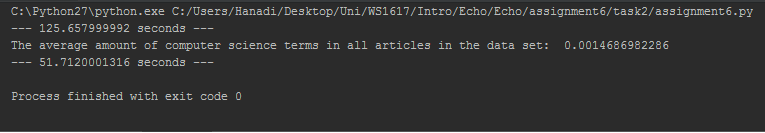
\includegraphics[width=1\textwidth]{output.png} \\ \\
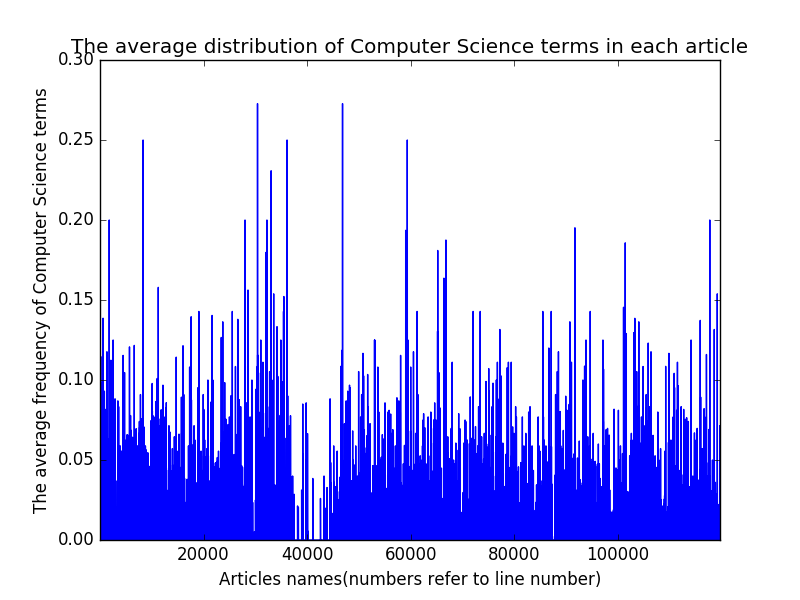
\includegraphics[width=1\textwidth]{figure_1.png} \\
% ------------------------------------------------------------------------------






\makefooter

\end{document}
